\documentclass[../discrete.tex]{subfiles}
\graphicspath{{\subfix{../figures/}}}
\begin{document}
\chapter{Logic and Proofs}
\section{Propositional Logic}
A proposition is a declarative statement that is either true or false.

For example, we can say there is a proposition $p$ and $q$, such as ``The sky is blue'' or ``The moon is made of cheese''. Something that is not a propositional statement is a statement that is neither true or false, such as ``Sit down'', which is just a statement. $x+1=2$ is not a propositional statement because it is either true or false, unless you assign a value for $x$.

A compound proposition is comprised of propositions and one or more of the following connectives:
\begin{itemize}
    \item negation: $\neg$ ``NOT'' ($\neg p$)
    \item conjunction: $\land$ ``AND'' ($p\land q$)
    \item disjunction: $\lor$ ``OR'' ($p\lor q$)
    \item implication: $\rightarrow$ ``IF, THEN'' ($p\rightarrow q$)
    \item biconditional $\leftrightarrow$ ``IF AND ONLY IF'' ($p\leftrightarrow q$)
\end{itemize}
Each proposition is represented by a propositional variable.

The negation of the proposition $p$ is $\neg p$ (not $p$). For example, If $p$ denotes ``The grass is green'', then $\neg p$ denotes ``it is not the case that the grass is green'', or ``the grass it not green''.
\begin{example}
    If $p$ is the statement ``my dog is the cutest dog'', then $\neg p$ is the statement ``my dog is not the cutest dog''.
\end{example}
\ex Negate the statement ``the door is not open.''
\ex Can you negate the statement ``Are we there yet?''

Truth Tables: Each row of a truth table gives us one possibility for the truth values of our proposition(s). Since each proposition has two possible truth values, true or false, we will have 2 rows for each proposition (or $2^n$ rows where $n$ is the number of propositions).

For $\neg p$, a truth table would look like 
\begin{tabular}{c|c}
    $p$ & $\neg p$\\ \hline
    T & F\\
    F & T
\end{tabular}
The left side is the combinations, and the right side is the connectives. For example, if we were looking at a truth table of $p\lor q$, the combinations would be $p$ and $q$, and the connectives would be $p\lor q$.

Conjunction: The conjunction of propositions $p$ and $q$ is denoted $p\land q$ and read $p$ ``and'' $q$. For a conjunction to be true, both propositions must be true.
The truth table looks like the following. 
\[\begin{tabular}{c|c|c}
    $p$ & $q$ & $p\land q$ \\ \hline 
    T & T & T \\\hline
    T & F & F\\\hline
    F&T&F\\\hline 
    F&F&F
\end{tabular}\]

Disjunction: The disjunction of propositions $p$ and $q$ is denoted $p\lor q$ and read $p$ ``or'' $q$. For a disjunction to be true, either proposition must be true.
\[ \begin{tabular}{c|c|c}
    $p$ & $q$ & $p\lor q$ \\ \hline
    T & T & T \\\hline
    T&F&T\\\hline
    F&T&T\\\hline
    F&F&F
\end{tabular}\]

The connective ``OR'' in English ``XOR''. The inclusive or is a disjunction $p\lor q$. The exclusive or is $p\oplus q$. Basically this is true only if one of the inputs is true, but not both or neither.
\[ \begin{tabular}{c|c|c|c}
    $p$ & $q$ & $p\lor q$ & $p\oplus q$\\ \hline
    T & T & T & F\\\hline
    T&F&T & T\\\hline
    F&T&T&T \\\hline
    F&F&F&F
\end{tabular}\]

Implication (Conditional Statement): The implication of propositions $p$ and $q$ is denoted $p\rightarrow q$ and read ``if $p$ then $q$'' or ``$p$ implies $q$''. 
When the hypothesis is true, the conclusion must be true for the implication to be true. WHen the hypothesis is false, the conclusion is true.
\[ \begin{tabular}{c|c|c}
    $p$ & $q$ & $p\rightarrow q$\\\hline 
    T & T & T\\\hline
    T & F & F\\\hline
    F&T&T\\\hline
    F&F&T 
\end{tabular}\]

From the implication $p\rightarrow q$, we can construct 3 news conditional statements.
\begin{itemize}
    \item Converse: $q\rightarrow p$ (Switch Order)
    \item Inverse: $\neg p\rightarrow \neg q$ (Negate),
    \item Contrapositive: $\neg q\rightarrow \neg p$ (Switch and Negative)
\end{itemize}
Contrapositives have the same truth value as $p\rightarrow q$.

\begin{example}
    Give the converse, inverse, and contrapositive of the implication: If your homework is complete, then your teacher is happy.

    The converse is, if the teacher is happy, then you completed your homework.

    The inverse is if you didn't complete your homework, then your teacher is not happy.

    The contrapositive is if your teacher is not happy, then you did not complete your homework.
\end{example}

Biconditional: The biconditional of propositions $p$ and $q$ is denoted $p\leftrightarrow q$ and read ``$p$ if and only if $q$''. 
For a biconditional to be true, both propositions must share the same truth value.
\[ \begin{tabular}{c|c|c}
    $p$ & $q$ & $p\leftrightarrow q$\\\hline
    T & T & T\\\hline
    T&F&F\\\hline
    F&F&T
\end{tabular}\]

The biconditional $p\leftrightarrow q$ can also be written as a compound proposition.
\[ (p\leftrightarrow q)\equiv (p\rightarrow q)\land (q\rightarrow p) \]
Can you show this?

The steps for constructing a truth table for compound propositions are as follows:

You need rows and columns. You need a row for every possible combination of values for the compound proposition. You need a column for each propositional variable, you need a column for the truth value of each expression that occurs in the compound proposition as it is built up, and you need a column for the compound proposition. The order of operations is as follows: $\neg, \land,\lor,\rightarrow,\leftrightarrow$.

\begin{example}
    Create a truth table for $(p\lor \neg q)\rightarrow (p\land q)$.

    \[ \begin{tabular}{c|c|c|c|c|c}
        $p$ & $q$ & $\neg q$ & $p\lor \neg q$ & $p\land q$ & $(p\lor\neg q)\rightarrow (p\land q)$\\\hline
        T & T & F & T & T & T\\\hline
        T&F&T&T&F&F\\\hline
        F&T&F&F&F&T\\\hline
        F&F&T&T&F&F
    \end{tabular}\]
\end{example}


\section{Propositional Equivalences}
Translating English Sentences:
\begin{enumerate}
    \item Identify atomic propositions.
    \item Determine appropriate logical connectives.
\end{enumerate}

For example consider the statement ``If I go to the store or the movies, I won't do my homework.''.

In that statement $p$ is going to the store, $q$ is going to the movies, and $r$ is doing homework, so $(p\lor q)\rightarrow \neg r$.

\ex Translate the propositional statement ``You can get a free sandwich on thursday if you buy a sandwich or a cup of soup.''

\ex Translate the propositional statement ``You can get a free sandwich on thursday only if you buy a sandwich or a cup of soup.''

\ex Translate the propositional statement ``The automated reply can't be sent when the system is full.'

Translating Propositions:
\begin{example}
    Let $q$ be ``You can ride the rollercoaster'', $r$ be ``You are under 4 feet tall'', and $s$ be ``you are older than 16 years old.''

    Translating $(r\lor \neg s)\rightarrow \neg q$ to english gives us, If $r$ or not $s$, then not $q$, or ``If you are under 4 feet tall or younger than 16 years old then you cannot ride the rollercoaster.''
\end{example}


\begin{example}
    An island has two kinds of inhabitants, knights, who always tell the truth, and knaves, who always lie. You go to the island and meet A and B. A says ``B is a knight''. B says, ``The two of us are opposite types.'' What are A and B? Let $p$ represent that A is a knight and $q$ represent that B is a knight.

    Using the propositional statements, $p\land q$, $p\land \neg q$, $\neg p \land q$, and $\neg p \land \neg q$, we can see that $\neg p \land \neg q$ satisfies the conditions that A and B are both knaves. (Note that this can also be done with a truth table.)
\end{example}

\ex When planning a party, you want to know whom to invite. Among the poeple you would like to invite are three touchy friends. You know that if Jasmine attends, she will become unhappy if Samir is there. Samir will attend only if Kanti will be there, and Kanti will not attend unless Jasmine also does. Which combinations of these three friends can you invite so as not to make someone unhappy?

Logic circuit - A circuit designed to perform complex tasks designed in terms of elementary logic functinos. Three `gates' are used used implementing a boolean function on one or more binary inputs producing one output.

The ``NOT GATE'' will have one input $p$, and output $\neg p$. The ``OR GATE'' will have two inputs, and output the disjunction of those two inputs. The ``AND GATE'' will have two inputs, and output the conjunction of the propositions. (Search up images yourself)

\section{Predicates and Quantifiers}
A tautology is a proposition which is always true. Ex. $p\lor \neg p$

A contradiction is a proposition which is always false. Ex. $p\land \neg p$

A contingency is a proposition which is neither a tautology nor a contradiction. Ex. $p$

Two compound propositions $p$ and $q$ are logically equivalent if $p\leftrightarrow q$ is a tautology, meaning they have the same truth value in all possible cases. This is written as $p\equiv q$, where $p$ and $q$ are compound propositions.

For example, the truth table below shows $\neg p\lor q\equiv p\rightarrow q$.
\[ \begin{tabular}{c|c|c|c|c}
    $p$ & $q$ & $\neg p$ & $\neg p\lor q$ & $p\rightarrow q$\\\hline
    T&T&F&T&T\\\hline
    T&F&F&F&F\\\hline
    F&T&T&T&T\\\hline
    F&F&T&T&T
\end{tabular}\]

\ex Determine if $\neg p\land q\equiv \neg p\lor \neg q$.

\ex Determine if $p\lor (q\land r)\equiv (p\lor q)\land (p\lor r)$.

Identity Laws:
\begin{itemize}
    \item $p\land T\equiv p$
    \item $p\lor F\equiv p$
\end{itemize}

Domination Laws:
\begin{itemize}
    \item $p\lor T\equiv T$
    \item $p\land F\equiv F$
\end{itemize}

Indempotent Laws:
\begin{itemize}
    \item $p\lor p\equiv p$
    \item $p\land p\equiv p$
\end{itemize}

Double Negation Law: $\neg(\neg p)\equiv p$

Absorbtion Laws:
\begin{itemize}
    \item $p\lor (p\land q)\equiv p$
    \item $p\land (p\lor q)\equiv p$
\end{itemize}

Negation Laws:
\begin{itemize}
    \item $p\lor \neg p\equiv T$
    \item $p\land \neg p\equiv F$
\end{itemize}

Commutative Laws:
\begin{itemize}
    \item $p\lor q\equiv q\lor p$
    \item $p\land q\equiv q\land p$
\end{itemize}

Associative Laws:
\begin{itemize}
    \item $(p\lor q)\lor r\equiv p\lor(q\lor r)$
    \item $(p\land q)\land r\equiv p\land(q\land r)$
\end{itemize}

Distributive Laws:
\begin{itemize}
    \item $p\lor (q\land r)\equiv(p\lor q)\land (p\lor r)$
    \item $p\land (q\lor r)\equiv (p\land q)\lor (p\land r)$
\end{itemize}

De Morgan's Laws:
\begin{itemize}
    \item $\neg(p\land q)\equiv \neg p\lor \neg q$
    \item $\neg(p\lor q)\equiv \neg p\land \neg q$
\end{itemize}

More equivalencies:
\begin{itemize}
    \item $p\rightarrow q\equiv \neg p \lor q$
    \item $p\rightarrow q\equiv \neg q\rightarrow \neg p$
    \item $p\lor q\equiv \neg p\rightarrow q$
    \item $p\land q\equiv \neg(p\rightarrow \neg q)$
    \item $(p\rightarrow q)\land (p\rightarrow r)\equiv p\rightarrow (q\land r)$
    \item $(p\rightarrow r)\land (q\rightarrow r)\equiv (p\land q)\rightarrow r$
    \item $(p\rightarrow q)\lor (p\rightarrow r)\equiv p\rightarrow (q\lor r)$
    \item $(p\rightarrow r)\lor (q\rightarrow r)\equiv (p\land q)\rightarrow r$
    \item $p\leftrightarrow q\equiv (p\rightarrow q)\land (q\rightarrow p)$
    \item $p\leftrightarrow q\equiv \neg p\leftrightarrow \neg q$
    \item $p\leftrightarrow q\equiv (p\land q)\lor (\neg p\land \neg q)$
    \item $\neg(p\leftrightarrow q)\equiv p\leftrightarrow \neg q$
\end{itemize}

We can construct new logical equivalences.
\begin{example}
    Show $\neg(p\lor (\neg p\land q))\equiv \neg p\land \neg q$ by developing a series of logical equivalences 
    
    The original statement is equivalent to $\neg p\land \neg(\neg p\land q)$ from the 2nd demorgan law.
    
    By the 1st De Morgan law, this is $\neg p\land \neg\neg p\lor \neg q$.

    Double negation: $\neg p\land (p\lor \neg q)$

    2nd Distributive Law: $(\neg p\land p)\lor (\neg p\land \neg q)$

    2nd Negation Law: $F\lor (\neg p\land \neg q)$

    Commutative Law for Disjunction: $(\neg p\land \neg q)\lor F$

    Identity Law: $\neg p\land \neg q$.
\end{example}

\ex Show $(p\land q)\rightarrow (p\lor q)$ is a tautology by developing a series of logical equivalences.

\ex Use logical equivalences to show $\neg(\neg p\lor q)\equiv \neg q\land p$


\section{Nested Quantifiers}
A nested quantifier is when one quantifier is in the scope of another.

Here is table that summarizes different quantifications involving two variables.
\begin{center}
    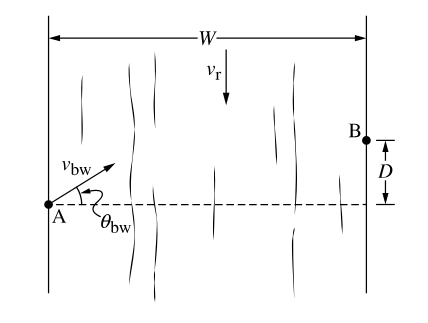
\includegraphics[width=1\textwidth]{1.5.PNG}
\end{center}

\section{Rules of Inference}
Rules of inference are our basic tools for establishing the truth of statements.

An argument in propositional logic is a sequence of propositions. All but the final proposition in the 
argument are called premises and the final proposition is called the conclusion. An argument is valid 
if the truth of all its premises implies the conclusion is true.

An argument form in propositional logic is a sequence of compound propositions involving propositional 
variables. An argument form is valid if no matter what particular propositions are substituted for the 
propositional variables in the premises, the conclusion is true if the premises are all true.

The tautology $(p\land(p\rightarrow q))\rightarrow q$ is the basis of the rule of inference 
modus ponens, or the law of detachment, basically: if $p$ and $p\rightarrow q \therefore q$.

Yet again another chart I took from Rosen.
\begin{center}
    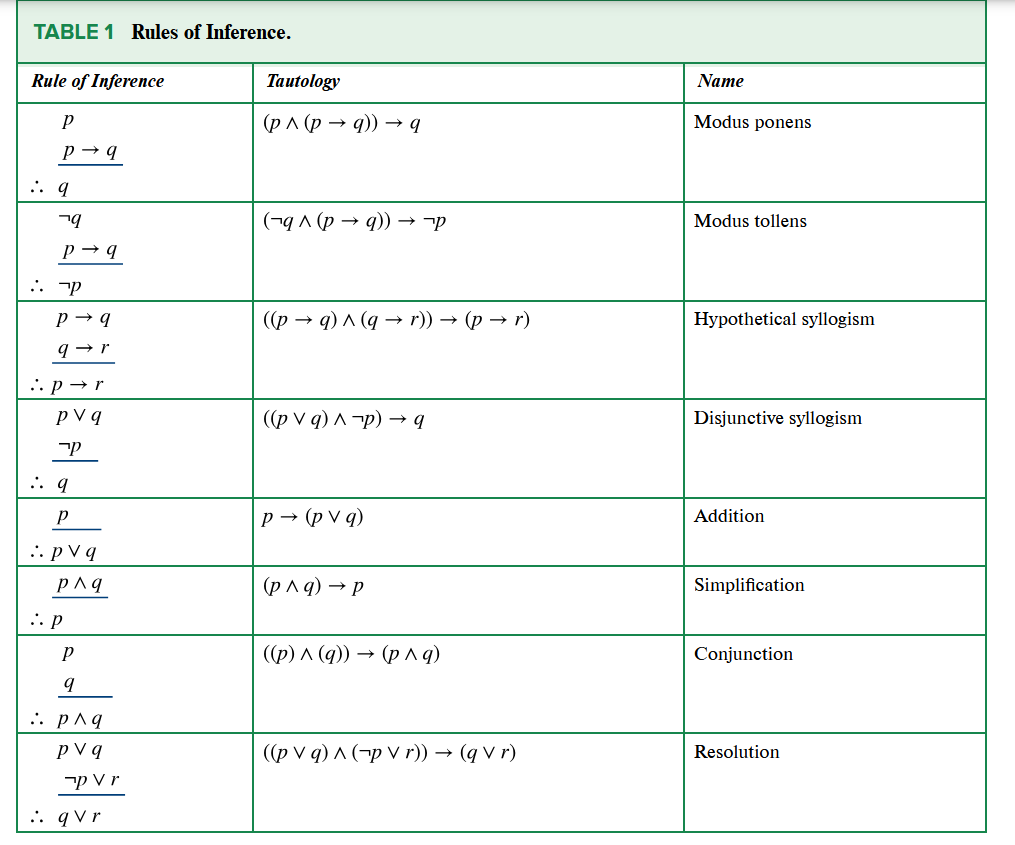
\includegraphics[width=1\textwidth]{1.6.PNG}
\end{center}

Fallacies resemble rules of inference, the difference lies in that they are based in contingencies rather than tautologies.

There are also some rules of inference for statements involving quantifiers.
This is what Rosen summarized:
\begin{center}
    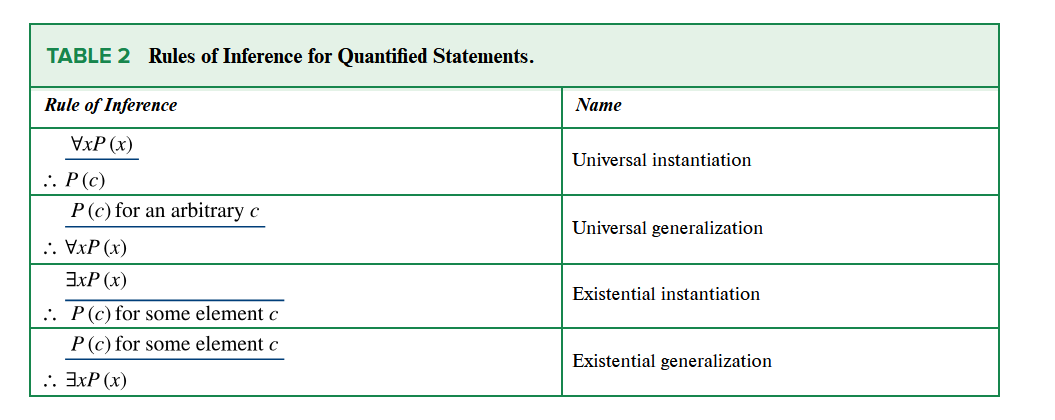
\includegraphics[width=1\textwidth]{1.6.1.PNG}
\end{center}

Because universal instantiation and modus ponens are so often used together, the combination of rules 
is called universal modus ponens. This rule tells us if $\forall x (P(x)\rightarrow Q(x))$ is true, 
and if $P(a)$ is true for a particular element $a$ in the domain of the universal quantifier, 
then $Q(a)$ must also be true. Note that by universal instantiation $P(a)\rightarrow Q(a)$ is true. 
By modus ponens, $Q(a)$ must also be true. 

This is how it is described:
\begin{center}
    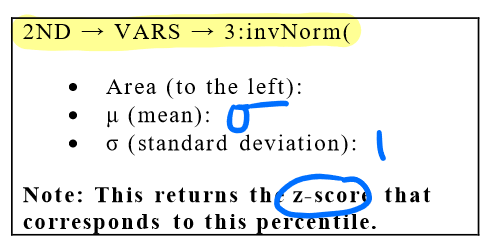
\includegraphics[width=0.5\textwidth]{1.6.2.PNG}
\end{center}

There is also universal modus tollens:
\begin{center}
    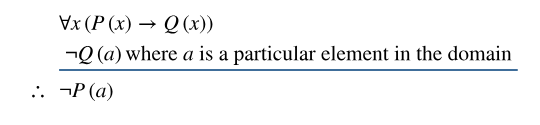
\includegraphics[width=0.5\textwidth]{1.6.3.PNG}
\end{center}

\section{Introduction to Proofs}
A proof is a valid argument that establishes the truth of a mathematical statement. 

A theorem is a statement that can be shown to be true. We show the truth using a proof.

A less important theorem that is helpful in the proof of other results is called a lemma. 

A corollary is a theorem that can be established directly from a theorem that has been proved. 

A conjecture is a statement that is being proposed to be a true statement.

A direct proof of a conditional statement $p\rightarrow q$ is constructed with the 
assumption that $p$ is true with the goal for the combination of $p$ being true and $q$ being false to never happen. 
\begin{definition}
    The integer $n$ is even if there exists an integer $k$ such that $n=2k$, and $n$ is odd if there exists an 
    integer $k$ such that $n=2k+1$. Two integers have the same parity when both are even or both are odd; they have 
    opposite parity when one is even and the other is odd.
\end{definition}

An indirect proof is a type of proof that is not direct. One example is proof by contraposition. P
roofs by contraposition use the fact that $p\rightarrow q$ is equal to $\neg q \rightarrow \neg p$. 
We have to show $\neg q \rightarrow \neg p$ is true to show that $p\rightarrow q$ is true as well.

We can prove that $p\rightarrow q$ is true if $p$ is false as well. This is called a vacuous proof. 

If we show that $q$ is true in $p\rightarrow q$ this is called a trivial proof. 
\begin{definition}
    The real number $r$ is rational if there exist integers $p$ and $q$ with $q\neq 0$ such that $r=p/q$. 
    A real number that is not rational is irrational.
\end{definition}

Suppose we want to prove a statement $p$ is true. Suppose that we can find a contradiction $q$ such that 
$\neg p \rightarrow q$ is true. Because $q$ is false, but $\neg p \rightarrow q$ is true, we can conclude 
$\neg p$ is false, meaning $p$ is true. 

To find a contradiction $q$ that might help us find that $p$ is true, we can show that 
$\neg p \rightarrow (r\land \neg r)$ is true for some proposition $r$. This is called a proof by contradiction. 

To prove a theorem in the form $p\leftrightarrow q$, we show that both $p\rightarrow q$ and $q\rightarrow p$ are both true. 

Many incorrect arguments are based on a fallacy called begging the question or circular reasoning. 
This fallacy occurs when one or more steps of a proof are based on the truth of the statement being proved.

\section{Proof Methods and Strategy}
Suppose we have a conditional $(p_1\lor p_2\lor \cdots \lor p_n)\rightarrow q$. We can separate the 
proof into different cases, called proof by cases by proving each of the $n$ conditional statements.

Some theorems can be proved by examining a relatively small number of examples. This is called proof by exhaustion. 

The phrase "without loss of generality" (WLOG) means that we assert by proving one case of a theorem, 
no additional argument is required to prove other specified cases. 

Many theorems are assertions that objects of a particular type exist. A theorem of this type is a 
proposition in the form $\exists xP(x)$, where $P$ is a predicate. A proof of a proposition in this 
form is called an existence proof. Sometimes an existence proof can be given by finding an element $a$, 
called a witness, such that $P(a)$ is true. This existence proof is called constructive. If we prove 
$\exists xP(x)$ is true in another way it can be nonconstructive.

For a uniqueness proof, we need two parts:
\begin{itemize}
    \item Existence: We show that an element $x$ with the desired property exists.
    \item Uniqueness: We show that if $x$ and $y$ both have the desired property, $x=y$
\end{itemize}

Forward reasoning is a proof when you start with your premises. You construct a proof with steps 
leading to the conclusion. It may sometimes be helpful to use backwards reasoning, we find a 
statement $p$ that we can prove $p\rightarrow q$. 
\end{document}